\documentclass[twosides]{memoir}
\usepackage{tikz-cd}
\usepackage{enumitem}
\usepackage{amsmath}
\usepackage{tabularray}
\usepackage{unicode-math}
\usepackage{ctex}
\usepackage{calc}
\usepackage{lipsum}
\usepackage{color,calc}
\usepackage{ninecolors}
\usepackage{tikz}
\usepackage{wallpaper}
\usepackage{titlesec}
\usepackage{tcolorbox}
\usepackage{fontspec}
\usepackage{mathtools}
\usepackage{mleftright}
\usepackage{amsthm}
\usepackage{pxrubrica}
\usepackage{hyperref}
\usepackage{multicol}


\usetikzlibrary{patterns}
\usetikzlibrary{arrows.meta}
\tcbuselibrary{skins}
\tcbuselibrary{breakable}
\tcbuselibrary{theorems}
\tcbuselibrary{most}
\let\left\mleft
\let\right\mright
\setcounter{tocdepth}{5}
\setsansfont{Noto Sans}

\makeatletter
\setcounter{tocdepth}{2}
\newCJKfontfamily\NotoSerifCJKJP{Noto Serif CJK JP}
\renewcommand{\cftchapteraftersnumb}{\hfill}
\renewcommand{\cftchapterfont}{\sffamily\large\bfseries}
\renewcommand{\cftchaptername}{{\scshape\large\chaptername}~}
\renewcommand{\cftchapterafterpnum}{\hspace*{-0.45ex}\par\vspace*{1em}}
\renewcommand{\cftchapterformatpnum}{\sffamily\large\bfseries\color{white}\colorbox{ChapBlue}}
\renewcommand*{\chapternumberline}[1]{\hspace*{-3em}\colorbox{ChapBlue}{\color{white}\cftchaptername #1}\cftchapteraftersnum\hfill\itshape\scshape\LARGE}

\renewcommand*{\cftsectionleader}{~\color{ChapBlue}\sffamily\small}
\renewcommand{\cftsectionfont}{\sffamily\scshape\small\bfseries}
\renewcommand{\cftsectionname}{{\small\bfseries\color{ChapBlue} \S}\space}
\renewcommand{\cftsectionafterpnum}{\cftparfillskip}
\renewcommand*{\cftsectionformatpnum}[1]{\sffamily\small{\large\special{pdf:literal direct 2 Tr 0.3 w }\color{ChapBlue}\(\longmapsto\kern-0.8em{\color{white}\special{pdf:literal direct 2 Tr 0.8 w }∎\special{pdf:literal direct 2 Tr 0.3 w }}\)\kern-1.5em\titlerule*[0.1pc]{\(-\)}\(\!\!\!\longrightarrow\)\special{pdf:literal direct 0 Tr 0 w }}~~\textit{#1}}

\renewcommand*{\cftsubsectionleader}{~\color{ChapBlue!20!white}\sffamily \titlerule*[0.2pc]{\(\cdot\)}}
\renewcommand{\cftsubsectionfont}{\footnotesize\slshape}
\renewcommand*{\cftsubsectionformatpnum}{~~\itshape\footnotesize\color{ChapBlue}}
\renewcommand{\cftsubsectionafterpnum}{\cftparfillskip\hspace*{2em}\par}



\newenvironment{defi}[2]{\mbox{}\\{\LARGE\({⌜}\)}\({}^{\color{ChapBlue}\symbf{DEF} }\)\hfill\textsf{\textbf{#1}}\\
    \slshape\small #2}{\mbox{}\hfill{\LARGE\(⌟\)}\par}

\renewenvironment{cases}[1]{\begin{dcases}#1}{\end{dcases}}

\newenvironment{thoerem}[2]{\begin{theo}{#1}{}\trivlist\item #2}{\end{theo}}

\newtcbtheorem[number within=section]{prof}{PROOF}{colback=ChapBlue!20,colframe=ChapBlue!150,fonttitle=\bfseries,arc=0mm,leftrule=0mm,toprule=0mm,bottomrule=1mm,rightrule=0mm,breakable}{prof}

\newtcbtheorem[number within=section]{theo}{THEOREM}{enhanced,title=My title,
    attach boxed title to top center=
        {yshift=-0.25mm-\tcboxedtitleheight/2,yshifttext=2mm-\tcboxedtitleheight/2},
    boxed title style={boxrule=0.5mm,
            frame code={ \path[tcb fill frame] ([xshift=-4mm]frame.west)
                    -- (frame.north west) -- (frame.north east) -- ([xshift=4mm]frame.east)
                    -- (frame.south east) -- (frame.south west) -- cycle; },
            interior code={ \path[tcb fill interior] ([xshift=-2mm]interior.west)
                    -- (interior.north west) -- (interior.north east)
                    -- ([xshift=2mm]interior.east) -- (interior.south east) -- (interior.south west)
                    -- cycle;}
        }, colback = ChapBlue!10!white, colframe = ChapBlue!50!black, sharp corners, colbacktitle = ChapBlue,fonttitle=\bfseries,coltitle=white}{theo}


\renewenvironment{quote}[2]{\begin{tcolorbox}[empty,
            coltitle=ChapBlue!75!black,fonttitle=\bfseries,
            borderline south={0.5mm}{0pt}{ChapBlue!50!white},
            title = {#1},
            titlerule style={ChapBlue,
                    arrows = {|-|}},
            leftrule = 0pt,
            rightrule = 0pt, breakable,
            colupper = darkgray
        ]\slshape\small\color{darkgray} #2}{\end{tcolorbox}}
\newfontface\ebgaramond{EB Garamond}
\usepackage[top=1.25in,bottom=1.3in,outer=1.3in,inner=1.3in]{geometry}
\newsavebox{\ChpNumBox}
\definecolor{ChapBlue}{rgb}{0.00,0.65,0.65}
\setmonofont{Iosevka}
\setCJKmainfont{Noto Serif CJK SC}[ItalicFont = FZKaiS-Extended]
\setCJKsansfont{Noto Sans CJK SC}[ItalicFont = FZKaiS-Extended]


\renewenvironment{proof}[2]{\begin{prof}{#1}{}\pushQED{\qed}\normalfont\topsep6\p@\@plus6\p@\relax\trivlist\item #2}{\popQED\endtrivlist\@endpefalse\end{prof}}
\providecommand{\xlongequal}[2][]{\ext@arrow 0099{\arrowfill@===}{#1}{#2}}
% \titleformat{\section}[display]
% {\vspace*{-3ex}}{\filright
%     \begin{tblr}{colspec = {c}, rows = {abovesep = 3pt,belowsep = -1pt}}
%         \SetCell{bg = ChapBlue!50!white, fg = ChapBlue!80!black}{\bfseries\LARGE\arabic{chapter}.\arabic{section}} \\
%         \vspace*{-2ex}\!\scshape\textit{Section}\!
%     \end{tblr}
%     \setcounter{subsection}{0}
%     \color{ChapBlue!70!black}\special{pdf:literal direct 2 Tr 0.5 w }\Large\(\longmapsto\kern-0.8em{\color{white}\special{pdf:literal direct 2 Tr 0.7 w }∎}\special{pdf:literal direct 2 Tr 0.5 w }\)\kern-1.5em\titlerule*[0.1pc]{\(-\)}\(\!\!\!\longrightarrow\)\special{pdf:literal direct 0 Tr 0 w }}{1em}{\vspace*{-5ex}\Large\bfseries\rightline}[\vspace{-3ex}]

\titleformat{\section}[hang]
{\vspace*{-3ex}}{\begin{tblr}{colspec = {c}, rows = {abovesep = 3pt,belowsep = -1pt}, row{2} = {abovesep = -5pt},baseline = T}
    \SetCell{bg = ChapBlue!50!white, fg = ChapBlue!80!black}{\bfseries\LARGE\arabic{chapter}.\arabic{section}} \\
    \makebox[0pt][c]{\scshape\textit{Section}}
\end{tblr}}{1em}{\color{ChapBlue!70!black}\special{pdf:literal direct 2 Tr 0.5 w}\LARGE\(\longmapsto\kern-0.8em{\color{white}\special{pdf:literal direct 2 Tr 0.9 w}∎}\special{pdf:literal direct 2 Tr 0.5 w}\)\kern-1.5em\titlerule*[0.1pc]{\(-\)}\(\!\!\!\longrightarrow\)\special{pdf:literal direct 0 Tr 0 w}~~\color{black}\Large\bfseries}[]

\newcommand{\abstractIN}{}

\newcommand{\newchap}[3]{
    \renewcommand{\abstractIN}{#3}
    \chapter[#1]{#2}\mbox{}\par
    \thispagestyle{forchapter}
    \setcounter{subsection}{0}
    \enlargethispage{-0.7in}
}



\titleformat{\subsection}[display]
{\vspace*{-1ex}}{}{}{\colorbox{ChapBlue!20!white}{\color{ChapBlue!90!black}\vspace{-3ex}\stepcounter{subsection}\large\bfseries\bfseries\thechapter.\arabic{section}.\arabic{subsection}}\hspace*{1em}\bfseries}


\makepagestyle{tocf}
\makeevenfoot{tocf}{}{\vskip5ex\colorbox{white}{\color{ChapBlue}~\bfseries\Roman{page}~}}{}
\makeoddfoot{tocf}{}{\vskip5ex\colorbox{white}{\color{ChapBlue}~\bfseries\Roman{page}~}}{}
\makeevenhead{tocf}{}{\ThisTileWallPaper{\paperwidth}{\paperheight}{tocOUT.pdf}}{}
\makeoddhead{tocf}{}{\ThisTileWallPaper{\paperwidth}{\paperheight}{tocIN.pdf}}{}
\makefootrule{tocf}{\textwidth}{2pt}{-9.6ex}
\makeheadfootruleprefix{tocf}{}{\color{ChapBlue}}

\makepagestyle{toc}
\makeheadrule{toc}{\textwidth}{0.4pt}
\makeevenfoot{toc}{}{\vskip5ex\colorbox{white}{\color{ChapBlue}~\bfseries\Roman{page}~}}{}
\makeoddfoot{toc}{}{\vskip5ex\colorbox{white}{\color{ChapBlue}~\bfseries\Roman{page}~}}{}
\makeoddhead{toc}{\ThisTileWallPaper{\paperwidth}{\paperheight}{tocIN.pdf}}{}{\scshape\sffamily 目录 \~{} Contents}
\makeevenhead{toc}{\scshape\sffamily 目录 \~{} Contents}{\ThisTileWallPaper{\paperwidth}{\paperheight}{tocOUT.pdf}}{}
\makefootrule{toc}{\textwidth}{2pt}{-9.6ex}
\makeheadfootruleprefix{toc}{}{\color{ChapBlue}}

\makepagestyle{fancy}
\makeevenfoot{fancy}{\vskip-8em\hspace{-2.5em}\rotatebox[origin=l]{90}{{\LARGE\ebgaramond ☙}\enspace{\bfseries\Roman{page}}\enspace{\LARGE\ebgaramond ❧}}}{}{}
\makeoddfoot{fancy}{}{}{\vskip-8ex\rotatebox[origin=r]{-90}{{\LARGE\ebgaramond ☙}\enspace{\bfseries\Roman{page}}\enspace{\LARGE\ebgaramond ❧}}\kern-2.5em}
\makeevenhead{fancy}{}{\leftmark}{}
\makeoddhead{fancy}{}{\rightmark}{}
\makeheadrule{fancy}{\textwidth}{0.4pt}

\makepagestyle{forchapter}
\makeevenfoot{forchapter}{\ThisTileWallPaper{\paperwidth}{\paperheight}{coverIN.pdf}}{\vskip10pt\color{white}\LARGE\textbf{\arabic{page}}}{}
\makeoddfoot{forchapter}{\ThisTileWallPaper{\paperwidth}{\paperheight}{coverIN.pdf}}{\vskip10pt\color{white}\LARGE\textbf{\arabic{page}}}{}



\newcommand*{\thickhrulefill}{%
    \leavevmode\leaders\hrule height 1\p@ \hfill \kern \z@}
\makechapterstyle{BlueBox}{%
    \setlength{\beforechapskip}{10pt}
    \setlength{\midchapskip}{26pt}
    \setlength{\afterchapskip}{20pt}
    \renewcommand{\printchaptername}{}
    \renewcommand{\chapternamenum}{}
    \def\chapternorthwest{}
    \def\chaptertitleIN{}
    \renewcommand{\printchapternum}{}
    \renewcommand{\printchaptertitle}[1]{\linespread{1}
        \noindent\begin{tblr}{width = \textwidth + 5em , colspec = {X[-1, c]X[h,l]}}
            \makebox[0pt][c]{\scshape Chapter} \strut                            & {\addtolength{\leftskip}{4ex}\thickhrulefill   \\  \Huge\bfseries ##1\strut\vspace*{-10em}}                                                                           \\
            \SetCell{bg=ChapBlue,fg=white,h,c}{\Huge\bfseries \thechapter\strut} & \SetCell{m}{\qquad\par\vspace*{2em}\TblrAlignBoth\addtolength{\leftskip}{2em}\setlength{\parindent}{2em}\slshape\linespread{1.3}\small\abstractIN \setlength{\parindent}{2em}} \\
        \end{tblr}
    }}

\makeatother
\makechapterstyle{toc}{%
    \setlength{\beforechapskip}{10pt}
    \setlength{\midchapskip}{26pt}
    \setlength{\afterchapskip}{20pt}
    \renewcommand{\printchaptername}{}
    \renewcommand{\chapternamenum}{}
    \def\chapternorthwest{}
    \def\chaptertitleIN{}
    \renewcommand{\printchapternum}{}
    \renewcommand{\printchaptertitle}[1]{
        \noindent\begin{tblr}{width = \textwidth, colspec = {X[-1, c]X[h,r]}}
            \makebox[0pt][c]{\scshape Chapter} \strut                                                                  & {\qquad \thickhrulefill \\ \qquad\Huge\bfseries ##1\strut\vspace*{-10em}} \\
            \SetCell{bg=ChapBlue,fg=white,h,c}{\rotatebox[origin=c]{90}{\color{white}\Huge\bfseries ~Contents~}\strut} &                                                                                    \\
        \end{tblr}
    }}


\titleformat{\paragraph}[runin]{\bfseries\color{ChapBlue}}{}{}{{\special{pdf:literal direct 2 Tr 0.3 w }\color{ChapBlue}\ebgaramond\char"261E}\hspace*{0.5em}\special{pdf:literal direct 0 Tr 0 w }}[]

\renewcommand{\contentsname}{目录\\ \LARGE Contents}

\AtBeginDocument{\addtocontents{toc}{\protect\thispagestyle{tocf}}}
\usetikzlibrary {lindenmayersystems}
   
\setmathfont{NewCMMath-Regular.otf}
\setmathfont[range = {"1D5A0-"1D63B, "1D5D4-"1D66F}]{Garamond-Math.otf}
\DeclareMathOperator{\id}{id}

\def\Obj{\operatorname{Obj}}
\def\Hom{\operatorname{Hom}}
\def\End{\operatorname{End}}
\def\Aut{\operatorname{Aut}}
\def\SET{\symsf{SET}}
\def\GRP{\symsf{GRP}}
\def\st{\text{ \underline{st} }}
\catcode`\。 = 13
\def。{.}
\setlist[enumerate]{label*=\arabic*., leftmargin = 0pt}
\setlist[itemize]{leftmargin = 0pt}
\everymath{\displaystyle}
\begin{document}

\setlength{\lineskip}{5pt}
\setlength{\lineskiplimit}{2.5pt}
\setlength{\parskip}{0.5em}

\setlist[itemize,2]{label = \(\circ\)}
\chapterstyle{toc}
\thispagestyle{empty}


\clearpage

\pagestyle{toc}\newgeometry{outer = 8cm, bottom = 6cm, top = 5cm, inner = 3cm}
\frontmatter
\tableofcontents*\restoregeometry
\clearpage
\linespread{1.3}

\pagestyle{fancy}

\mainmatter
\chapterstyle{BlueBox}
\setcounter{page}{1}


\newchap{Preliminaries}{Preliminaries: \\
    Set theory \& categroies}{}


\section{Naive set theory}


\subsection{集合的运算}

\begin{defi}{集合的运算}
    \begin{itemize}
        \item \(\cup:\) union;
        \item \(\cap:\) intersection;
        \item \(\backslash:\) difference;
        \item \(\amalg :\) disjoint union;
        \item \(\times :\) set product;
    \end{itemize}
\end{defi}

\subsection{disjoint union}


\begin{defi}{Disjoint union}
    \(S \amalg T\):得到 \(S\) 与 \(T\) 的拷贝 \(S'\) 与 \(T'\),且 \(S' \cap T' = \varnothing\),则 \(S' \cup T' = S\amalg T\)。
    其中一种依赖于 set product 的实现:
    \[
        \begin{cases}
            S' \coloneqq \left\{ 0 \right\} \times S, \\
            T' \coloneqq \left\{ 1 \right\} \times T.
        \end{cases}
    \]
\end{defi}

\subsection{set product}

\begin{defi}{Set product}
    \[
        S \times T\coloneqq \left\{ \left\{ \left\{ s \right\} ,\left\{ s,t \right\}  \right\} : s\in S\land t\in T \right\}
        .\]

    将 \(\left\{ \left\{ s \right\} ,\left\{ s,t \right\}  \right\}\) 写作 \((s,t)\),称为 pair。
\end{defi}
\subsection{等价关系}


\begin{defi}{等价关系}
    若 \(\symcal{R} \) 是二元关系,则 \(a,b\) 满足关系 \(\symcal{R} \) 写为:
    \[
        a\mathop{\symcal{R}}b
        .\]

    若关系 \(\sim\) 定义在集合 \(S\)上满足:
    \begin{itemize}
        \item reflexivity: \((\forall a\in S) a \sim a\).
        \item symmetry: \((\forall a\in S)(\forall b\in S) a\sim b \implies b \sim a\).
        \item transitivity: \((\forall a\in S)(\forall b\in S)(\forall c\in S) a\sim b \land b\sim c \implies a\sim c\).
    \end{itemize}
    则称 \(\sim\) 是在集合 \(S\) 上的等价关系。
\end{defi}


\subsection{分划与等价类 (partition \& equivalence class)}

\begin{defi}{分划与等价类}
    \begin{itemize}
        \item \textbf{分划}是一个集合的集合,满足:
              \[
                  \begin{cases}
                      (\forall a\in P) (\forall b \in P) a \cap b = \varnothing, \\
                      \bigcup_{a \in P} a = S.
                  \end{cases}
              \]
              则称 \(P\) 是 \(S\) 的分划。
        \item \textbf{等价类}:
              \[
                  [a]_{\sim} \coloneqq  \left\{ x \in S : x \in a \right\}
                  .\]
              称此为在 \(S\) 上 \(a\) 的等价类,由于等价类两两不交,且具有自反性,则 \(S\) 上某等价关系得到的所有等价类组成的集合是 \(S\) 的分划 \(\symcal P_{\sim}\)。
    \end{itemize}
\end{defi}


\subsection{集合商 (set quotient)}
\begin{defi}{集合商}
    集合 \(S\) 与等价关系 \(\sim\) 的商定义为:
    \[
        S /\mathord \sim \coloneqq\symcal{P} _{\sim}
        .\]
\end{defi}

即 \(a,b\in S\) 等价 \(\iff\) 商到同一个元素。

\begin{quote}{一个集合商的例子}
    定义 \(\symbb{Z} \) 上的等价关系 \(\sim\) : \(a\sim b \iff \frac{a - b}{2} \in\symbb{Z}\),则:
    \[
        \symbb{Z} /\mathord \sim = \left\{ [0]_{\sim} , [1]_{\sim} \right\}
        .\]
\end{quote}


\section{Functions between sets}


\subsection{函数}

\begin{defi}{函数}
    \begin{itemize}
        \item 函数的 Graph:
              \[
                  \Gamma _f \coloneqq \left\{ (a,b) \in A \times B : b = f(a) \right\}
                  .\]
              且满足 \((\forall a\in A)(\exists !b\in B) (a,b) \in \Gamma_f \),即 \((\forall a\in A)(\exists !b\in B) f(a) = b\)。
        \item 函数的图的表示:

              \[
                  \begin{cases}
                      A \xrightarrow{f} B, \\
                      a \mapsto f(a).
                  \end{cases}
              \]
    \end{itemize}
\end{defi}

\subsection{Indentity function(id)}

在集合 \(A\) 上有:
\[
    \id_A : A\to A , (\forall a\in A)\id_A(a) = a
    .\]
\subsection{函数的 image}

若 \(S\subset A, f : A \to B\),则:

\[
    f(S) \coloneqq \left\{ b\in B : (\exists a \in S) f(a) = b  \right\}
    .\]

则 \(f(A)\) 就是函数的image,记作 \(\operatorname{im}f\)

\subsection{函数的 restriction}

记 \(S\subset A\),则:
\[
    f|_S : S \to A, (\forall s\in S) f|_S(s) = f(s)
    .\]

\subsection{函数的复合 (composition)}

\begin{itemize}
    \item 若 \(f:A\to B, g: B\to C\),则 \(g\circ f: A\to C, (\forall a\in A) g\circ f(a) \coloneqq g\left( f(a) \right) \)。
\end{itemize}
\[
    \begin{tikzcd}
        A \arrow[rd, "g \circ f"]\arrow[r, "f"] & B\arrow[d, "g"] \\
        {}                                      & C
    \end{tikzcd}
\]
{\slshape 此时称图是交换(commutative)的,因为图描述的所有从 \(A\) 到 \(C\) 的通路都会送 \(A\) 中的任意一个元素到相同的结果。 }

函数的复合满足结合律:
\[
    \begin{tikzcd}
        A\arrow[r, "f"]\arrow[rr, "g\circ f", bend left = -40] & B\arrow[r, "g"]\arrow[rr, "g\circ f", bend left = 40] & C\arrow[r, "h"] & D
    \end{tikzcd}
    .\]
即 \(h \circ (g \circ f) = (h\circ g) \circ f\)。

\subsection{单射、全射、双射(injections, surjections, bijections)}


\begin{defi}{单射 (Injections, \textbf{Inj})}
    \(f: A\to B\) 是单的若:
    \[
        (\forall a'\in A)(\forall a''\in A) a' \neq a'' \implies f\left( a' \right) \neq f(a'')
        .\]
    实际上就是 \((\forall a'\in A)(\forall a''\in A) f\left( a' \right) = f\left( a'' \right) \implies a'=a''\)。
    一般用箭头 \(f: A ↪ B \) 表示。
\end{defi}

\begin{defi}{全射 (Surjections, \textbf{Surj})}
    \(f : A\to B\) 是全的若:
    \[
        (\forall b\in B)(\exists a\in A) f(a) = b
        .\]
    此时 \(\operatorname{im}f = B\)。
    一般用箭头 \(f: A ↠ B\) 表示。
\end{defi}

\begin{defi}{双射 (Bijections, \textbf{Bij})}
    \(f\) 是双的当且仅当 \(f\) 又单又全,一般用箭头 \(f: A\stackrel{\sim}{\to }B\) 表示。
    \begin{itemize}
        \item 若 \(\exists f: A \stackrel{\sim}{\to } B\),则记此时 \(A\cong B\),若其中一个集合元素数量有限,则另一个也有限且两个集合元素数量相等。
        \item 集合 \(A\) 中的元素数量写作 \(|A|\);幂集写作 \(2^A\)。
    \end{itemize}
\end{defi}

\subsection{单射、全射、双射的性质}
\begin{itemize}
    \item 双射有逆 (inverse):
          \begin{theo}{双射有逆}{}
              定义函数 \(f: A\stackrel{\sim}{\to }B\),定义 \(g: B \to 2^A, (\forall b\in B)g(b) = \left\{ a : f(a) = b \right\} \),则由于 \(f\) 是单的,则 \((\forall a',a''\in A)f(a') = f(a'') \implies a' = a'\),故 \((\forall b\in B ) |g(b)| = 1\)。故可以定义 \(g': B \to A, (\forall b\in B) g(b) = a, \text{ \underline{st} } f(a) = b\),且是良定义的。

              此时 \(g'\circ f = \id_A, f\circ g' = \id_B\),此称 \(g'\) 为 \(f\) 的逆,记为 \(f^{-1} \)。
          \end{theo}

          双射的逆唯一:
          \begin{proof}{双射的逆唯一}
              定义 \(f : A \stackrel{\sim}{\to} B\) 的逆 \(g,g'\),由于 \(f\circ\id_A = f = \id_B\circ f\),因此:
              \[
                  g = g\circ \id_B = g\circ (f \circ g') = (g \circ f) \circ g' = \id_A \circ g' = g'
                  .\]
              故唯一。
          \end{proof}
    \item 左逆与右逆 (Linv \& Rinv)
          若 \(f: A\to B, g\circ f = \id_A\),则称 \(g\) 是 \(f\) 的左逆,同理有右逆。

          如果 \(A \neq \varnothing, f:A\to B\):
          \begin{itemize}
              \item \(f\) 有 Linv \(\iff f\) 是单的。
                    \begin{proof}{}
                        \begin{enumerate}
                            \item (\(\implies \)) 若 \(f\) 有左逆,设为 \(f^{-1} \),则:
                                  \[
                                      (\forall a,b\in A\land a\neq b)f^{-1} (f(a)) = \id_A(a) = a \neq b = f^{-1} (f(b))
                                      .\]
                                  若 \((\exists a,b\in A)f(a) = f(b)\),则与上式矛盾,故 \(f\) 是单的。
                            \item (\(\impliedby \)) 若 \(f\) 是单的,有双射有逆那部分的讨论知道 \((\forall b\in\operatorname{im}f)\exists !a \in A \text{ \underline{st} } f(a) = b\),故定义:
                                  \[
                                      g(b)\coloneqq \begin{cases}
                                          a, & \text{if }(\exists a\in A)b = f(a),    \\
                                          S, & \text{if } b \notin \operatorname{im}f.
                                      \end{cases}
                                  \]
                                  则 \(g\) 满足 \(g\circ f = \id_A\)。
                        \end{enumerate}
                    \end{proof}
              \item \(f\) 有 Rinv \(\iff f\) 是全的。
                    \begin{proof}{}
                        只证明 \((\impliedby )\) 的部分,由于 \(f\) 是全的,定义:
                        \[
                            g:B\to 2^A, b\mapsto  \left\{ a\in A : f(a) = b\right\}
                            .\]
                        则 \((\forall b\in B)g(b) \neq \varnothing\),定义:
                        \[
                            h:B\to A, b \mapsto a \text{ \underline{st} } a   \in g(b)
                            .\]
                        这样定义的 \(h\) 可能有很多种,但都满足其是 \(f\) 的右逆:
                        \[
                            (\forall b\in B)h(b) \in g(b) \implies f\circ h(b) = \id_B
                            .\]
                    \end{proof}
              \item 若\(f\)同时有左逆和右逆,则两个逆相同。
          \end{itemize}
\end{itemize}
\begin{quote}{一些单射、全射的例子}
    \begin{itemize}
        \item 投影
              \[
                  \begin{tikzcd}
                      {} & A\times B\arrow[rd, "\pi_B", two heads]\arrow[ld, "\pi_A"', two heads] & {} \\
                      A  & {}                                                                     & B  \\
                  \end{tikzcd}
              \]
              其中 \(\pi \) 是投影 (projection) 映射:
              \[
                  \begin{aligned}
                      \pi _A((a,b)) \coloneqq a , \\
                      \pi _B((a,b))\coloneqq b.
                  \end{aligned}
                  .\]
              是全射。

        \item 与不交并的映射
              \[
                  \begin{tikzcd}
                      A\arrow[rd, "f_B",hook] & {}         & B\arrow[ld, "f_A"', hook'] \\
                      {}                      & A\amalg  B & {}                         \\
                  \end{tikzcd}
              \]
              若将 \(A\amalg B\) 表示为 \(A'\cup B'\),其中 \(A'\overset{F_A}{\cong} A, B'\overset{F_B}\cong B\),则 \((\forall a\in A)f_A(a) \coloneqq F_A(a) \in A\amalg B\)。
        \item 商
              \[
                  \begin{tikzcd}
                      A\arrow[r, "f", two heads] & A /\mathord \sim
                  \end{tikzcd}
              \]
        \item 函数的标准分解 (Canonical decomposition)
              对函数 \(f:A\to B\),在 \(A\) 上建立等价关系:
              \[
                  a\sim b \iff f(a) = f(b)
                  .\]
              则函数可以分解为:
              \[
                  \begin{tikzcd}
                      A\arrow[r, two heads]\arrow[rrr, bend left = 40, "f"] & A /\mathord \sim \arrow[r, "\sim", "\tilde f"'] & \operatorname{im}f\arrow[r, hook] & B
                  \end{tikzcd}
              \]
              其中 \(\tilde f:A / \mathord\sim \to \operatorname{im} f, \tilde f([a]_{\sim}) \coloneqq f(a)  \),不难验证这是良定义的,现在证明 \(\tilde f\) 是双射:
              \begin{proof}{}
                  只需证明 \(f\) 既是单射也是全射就可以了:
                  \begin{enumerate}
                      \item \textbf{inj}:
                            \[
                                \tilde f\left( [a]_{\sim} \right)  = \tilde f\left( [b]_{\sim} \right) \implies f(a) = f(b) \implies a\sim b \implies [a]_{\sim} = [b]_{\sim}
                                .\]
                      \item \textbf{surj}:
                            \[
                                (\forall b\in \operatorname{im}f)\exists a\in A \text{ \underline{st} }f(a) = b \implies \tilde f\left( [a]_{\sim} \right) = b
                                .\]
                  \end{enumerate}
              \end{proof}
    \end{itemize}
\end{quote}


\section{范畴 (Categories)}



一个范畴 \(\symsf C\)包括:
\begin{itemize}
    \item 一个类 \(\Obj(\symsf C)\),包括了对象 (object)。
    \item 对任意两个对象 \(A,B\) 存在一个集合记为 \(\Hom_{\symsf C}(A,B)\) 包含了从 \(A\) 到 \(B\) 的全部态射 (morphisms),态射和 \(\Hom\) 满足以下特点:
          \begin{itemize}
              \item \textbf{幺元的存在性}

                    \(\forall A\in \symsf C,\exists 1_A \in \Hom_{\symsf C}(A,A) \eqcolon \End_{\symsf C}(A)\),称为 \(A\) 的 indentity。
              \item \textbf{态射复合的存在性}

                    若 \(\exists f\in \Hom_{\symsf C}(A,B), g\in \Hom_{\symsf C}(A,B)\),则存在 \(f,g\) 决定的态射 \(gf\in \Hom_{\symsf C}(A,C)\),由于 \(\Hom\) 是集合,因此存在函数:
                    \[
                        \Hom_{\symsf C}(A,B) \times \Hom_{\symsf C}(B,C) \to \Hom_{\symsf C}(A,C)
                        .\]
              \item \textbf{态射复合的结合性}

                    若 \(f\in \Hom_{\symsf C}(A,B), g\in \Hom_{\symsf C}(B,C), h\in \Hom_{\symsf C}(C,D)\),则
                    \[
                        (hg)f = h(gf)
                        .\]
                    这一性质导致态射图可交换。
              \item \textbf{幺元律}

                    \[
                        \forall f\in \Hom_{\symsf C}(A,B),f 1_A = 1_Bf=f
                        .\]
          \end{itemize}
\end{itemize}

\begin{quote}{一些范畴的小例子}
    \begin{enumerate}[label = \textbf{\arabic*.}]
        \item 对象为集合、态射为集合函数的范畴,记为 \(\SET\):
              \begin{itemize}
                  \item \(\Obj(\SET) \coloneqq \) 一个包含所有集合的类。
                  \item \(\Hom_{\SET}(A,B) \coloneqq B^A\)。
              \end{itemize}
        \item 一个关于二元运算的范畴:若 \(S\) 上的二元运算 \(\sim\) 满足:
              \[
                  (\forall a,b,c\in S)\begin{cases}
                      a\sim a, \\
                      a\sim b\land b\sim c\implies a\sim c .
                  \end{cases}
              \]
              则定义 \(\symsf C_{\sim}\):
              \begin{itemize}
                  \item \(\Obj\left( \symsf C_{\sim} \right) \coloneqq S\)。
                  \item \(\Hom_{\symsf C_{\sim}}(A,B)\coloneqq \begin{cases}
                            (A,B),       & \text{if }A\sim B,  \\
                            \varnothing, & \text{if }A\nsim B.
                        \end{cases}\)
              \end{itemize}
              定义复合为:
              \[
                  \circ _{\symsf C_{\sim}} :((A,B),(B,C))\mapsto (A,C)
                  .\]
              则其为一个范畴。
              \begin{itemize}
                  \item 一个特例,如果认为 \(S=\symbb{Z} \),\(\sim\) 为 \(\leqslant \),则态射图如下:
                        \[
                            \begin{tikzcd}
                                2\arrow[r]\arrow[rd] & 3\arrow[r]\arrow[d, "1_3"] & 4\arrow[r]  & 5  \\
                                {}                   & 3\arrow[r]\arrow[rru]      & 4\arrow[ru] & {}
                            \end{tikzcd}
                        \]
              \end{itemize}
        \item \textbf{由范畴诱导范畴}
              \begin{itemize}
                  \item [\scshape\bfseries Slice CAT]
                        考虑范畴 \(\symsf C\) 中的对象 \(A\),接下来构建 \(\symsf C_A\):
                        \begin{itemize}
                            \item \(\Obj(\symsf C_A) \coloneqq \)  \(\symsf C\) 中所有到 \(A\) 的态射。
                            \item \(\Hom_{\symsf C_A}(f_1,f_2) = \left\{ \sigma :f_1=f_2 \sigma  \right\} \)。
                        \end{itemize}
                        \[
                            \begin{tikzcd}
                                Z_1\arrow[d, "f_1"']\arrow[rd, "\sigma "] & {}                    \\
                                A                                         & \arrow[l,"f_2"']  Z_2 \\
                            \end{tikzcd}
                        \]
                        \(\symsf C_A\) 中态射的复合取自 \(\symsf C\) 中的态射复合。
                  \item [\scshape\bfseries CoSlice CAT]
                        同理,只不过将从到 \(A\) 变成了 \(A\) 到其他对象的态射。
                  \item [\scshape\bfseries Opp CAT]
                        \begin{itemize}
                            \[
                                \begin{cases}
                                    \Obj(\symsf C^{\symup{op}})\coloneqq \Obj(\symsf C), \\
                                    \Hom_{\symsf C^{\symup{op}}}(A,B)\coloneqq \Hom_{\symsf C}(B,A).
                                \end{cases}
                            \]
                        \end{itemize}
              \end{itemize}
    \end{enumerate}
\end{quote}


\subsection{态射们}



\begin{defi}{同构 (Isomorphisms)}
    若一个态射 \(f \in \Hom_{\symsf C}(A,B)\) 满足:
    \[
        \exists g\in \Hom_{\symsf C}(B,A) \st gf=1_A, fg=1_B
        .\]
    则 \(f\) 是一个同构,此时记 \(g\) 为 \(f^{-1} \),如果 \(f\) 有左逆、右逆,则它们必然相等(唯一)。
\end{defi}

\begin{quote}{一些关于逆相关范畴的例子}
    \begin{itemize}
        \item 一个同构都是 indentity 的例子,用 \((\symbb{Z} ,\leqslant )\)定义的范畴。
        \item 一个每个态射都是同构的例子,用 \((\symbb{Z} ,=)\) 定义的范畴。这种性质的范畴被称为广群 (Groupoids)。
    \end{itemize}
\end{quote}

\begin{defi}{自同构 (Automorphisms)}
    就是属于 \(\End\) 的同构,所有 \(A\) 的自同构组成的集合称为 \(\Aut_{\symsf C}(A)\)。
    \begin{itemize}
        \item \(f,g \in\Aut_{\symsf C}(A) \implies fg\in\Aut_{\symsf C}(A)\)。
        \item \(f\in \Aut_{\symsf C}(A) \implies f^{-1} \in\Aut_{\symsf C}(A)\)。
    \end{itemize}
    \(\Aut\) 是一个\textbf{群} (Group)。
\end{defi}

\begin{defi}{单态射 (Monomophisms, \textbf{Monic})}
    即满足左消去律的态射:
    \begin{gather*}
        \forall Z\in \Obj(\symsf C),\forall a,b\in\Hom_{\symsf C}(Z,A),f:A\to B\\
        f \textup{ is a monic} \iff \left( f\circ a=f\circ b \implies a=b \right)
    \end{gather*}
\end{defi}

\begin{defi}{全态射 (Epimorphisms, \textbf{Epic})}
    满足右消去律的态射:
    \begin{gather*}
        \forall Z\in \Obj(\symsf C),\forall a,b\in\Hom_{\symsf C}(B,Z) ,f:A\to B\\
        f \textup{ is an epic} \iff \left( a\circ f=b\circ f \implies a=b \right)
    \end{gather*}
\end{defi}


在 \(\SET\) 中,单态射和全态射就是集合之间的单射和全射。

\begin{proof}{\(\SET\)中的单/全态射是集合之间的单/全射}
    \((\impliedby) \),只需考虑单/全射的左/右逆即可:
    \[
        f\circ a=f\circ b\implies f^{-1} \circ f\circ a=f^{-1} \circ f\circ b\implies a=b
        .\]

    \((\implies)\),可以用反证法,若 \(f\) 是非单射但是是单态射,则 \(\exists a\neq b(f(a)=f(b))\),考虑态射 \(A:\left\{ * \right\} \to a,B:\left\{ * \right\} \to b\),则 \( A \neq B\land f\circ A = f\circ B\),与单态射的定义矛盾。

    类似的,若 \(f:A\to B\) 是非全射且是全态射,则 \(B\backslash {\operatorname{\symrm{im}}f}\neq \emptyset\),定义态射 \(X: B\to \left\{ 1 \right\} ,Y:B\to \left\{ 0,1 \right\}\),且:
    \[
        Y(y)\coloneqq \begin{cases}
            1,  & \text{if }y\in \operatorname{im}f ,   \\
            0 , & \text{if }y \notin\operatorname{im}f.
        \end{cases}
    \]
    则同样与全态射的定义矛盾。
\end{proof}

\textbf{注意!Iso 并不等于 Monic \(\land\) Epic!}具体例子可以见 \((\symbb{Z} ,\leqslant )\)所定义的范畴:每个 \(\Hom\) 中只有一个态射,则必然左/右可消去,但只有 \(\End\) 是同构。同时,Monic的复合是Monic,Epic同理。


\section{泛性质(Universal properties)}

泛性质与 I(nitial) / F(inal) 对象有关:

\begin{defi}{I 对象与 F 对象}
    \(A\in\Obj\left( \symsf C \right) \),则 \(A\) 是 I 的若:
    \[
        (\forall Z\in\Obj(\symsf C))\left\vert \Hom_{\symsf C}(A,Z) \right\vert =1
        .\]
    \(A\) 是 F 的若:
    \[
        (\forall Z\in\Obj(\symsf C))\left\vert \Hom_{\symsf C}(Z,A) \right\vert =1
        .\]
    若 \(I_1,I_2\) 是 \(\symsf C\) 上的 I / F 对象,则 \(I_1\cong I_2\)。
\end{defi}


\subsection{泛性质与一些例子}

泛性质长得像一个范畴的 I/F 对象,比如:

\begin{quote}{空集的泛性质是「集合之间的映射」}
    因为以集合为对象、集合映射为态射的范畴 \(\SET\) 中,空集是 I 对象。
\end{quote}

\begin{quote}{一些其他例子}
    \begin{itemize}
        \item 集合商 \(A / \mathord\sim\) 的泛性质是从集合 \(A\) 到其他映射集合的映射,满足:“等价的 \(A\)中元素有相同的像。”
              即
              \[
                  A\xrightarrow{f}Z, f\st a\sim b \implies f(a) = f(b)
                  .\]
              以此为范畴 \(\symsf C_{A,\sim}\) 的 \(\Obj\),则态射为 \(\Hom(f_1,f_2) = \left\{ \sigma :\sigma f_1=f_2 \right\} \),则考虑以下cd:
              \[
                  \begin{tikzcd}
                      A/\mathord \sim\arrow[r, "\exists !\sigma"]          & Z  \\
                      A \arrow[u, "\pi"]\arrow[ur, "f_A", bend right = 20] & {}
                  \end{tikzcd}
              \]
              其中 \(\pi \) 已给定(为商投影映射),则 \(A/\mathord\sim\) 是这个范畴的 I 对象。
              \begin{proof}{}
                  \(\forall a\in A\) 都有 \(\sigma \pi (a) = f_A(a)\),即 \(\sigma \left( [a]_{\sim} \right) = f_A(a) \),此就相当于定义了 \(\sigma\)(保证唯一),易证 \(\sigma\) 是良定义的。
              \end{proof}
              同时,\(\operatorname{im}f\) 也是其 I 对象:
              \[
                  \begin{tikzcd}
                      \operatorname{im}f \sim\arrow[r, "\exists !\sigma'"] & Z  \\
                      A \arrow[u, "f"]\arrow[ur, "f_A", bend right = 20]   & {}
                  \end{tikzcd}
              \]
              故由 I 对象的特点有 \(\operatorname{im}f \cong A / \mathord\sim\)。
        \item 集合的积
              集合 \(A,B\) 的积的泛性质是一个集合到 \(A\) 和 \(B\) 的两个映射。

              给出三元组 \((Z,f_A,f_B)\),此为 \(\symsf C\) 的 \(\Obj\)。则其态射为:
              \[
                  \Hom\left( (Z_1,f_A,f_B),(Z_2,g_A,g_B) \right) \coloneqq \left\{ \sigma:g_A\sigma = f_A\land g_B\sigma = f_B \right\}
                  .\]
              \(A\times B\)是其 F 对象:
              \[
                  \begin{tikzcd}
                      {}                                                                & A  & {}                                                  \\
                      Z\arrow[ur, "f_A"]\arrow[dr, "f_B"']\arrow[rr, "\exists !\sigma"] & {} & A\times B \arrow[ul, "\pi _A'"]\arrow[ld, "\pi _B"] \\
                      {}                                                                & B  & {}
                  \end{tikzcd}
              \]
              对 \(\forall z\in Z\) ,都有:
              \[
                  \begin{cases}
                      \pi _A\sigma (z) = f_A(z), \\
                      \pi _B\sigma(z) = f_B(z).
                  \end{cases}
              \]
              故 \(\sigma : z\mapsto \left( f_A(z), f_B(z) \right) \),唯一。

              定义 \(A \times B\) 中的积 (product) 为 \(\symsf C_{A,B}\) 那个的 F 对象(若存在)。
              \begin{itemize}
                  \item 另一个例子,在 \(\symbb{Z}, \leqslant \) 定义的范畴中, \(A\times B\coloneqq \min(A,B)\)。
              \end{itemize}
        \item 余积 (Coproduct)
              定义 \(A,B\)余积 \(A\amalg B\)为 \(\symsf C^{A,B}\) 中的 I 对象,则 \(\SET\) 中的余积为两个集合的不交并。

              \begin{proof}{}
                  \[
                      \begin{tikzcd}
                          {}                                  & A\amalg B \arrow[dd, "\exists !\sigma"] & {}                                  \\
                          A\arrow[ru, "I_A"]\arrow[rd, "f_A"] & {}                                      & B\arrow[ul, "I_B"]\arrow[ld, "f_B"] \\
                          {}                                  & Z                                       & {}
                      \end{tikzcd}
                  \]
                  如图所示,考虑 \(A \amalg B\) 的一种实现:
                  \[
                      A\cong A',B\cong B',A'\cap B'=\varnothing,A'\cup B'\cong A\amalg B
                      .\]
                  则,\(\begin{cases}
                      \forall a\in A, \sigma I_A(a) = f_A(a) \\
                      \forall b\in B, \sigma I_B(b) = f_B(b)
                  \end{cases}\),故:
                  \[
                      \sigma : a\mapsto \begin{cases}
                          f_A\left( I_A^{-1} |_{A'} (a) \right) , & \text{if } a \in A', \\
                          f_B\left( I_B^{-1} |_{B'} (b) \right) , & \text{if } a \in B'.
                      \end{cases}
                  \]
              \end{proof}
    \end{itemize}
\end{quote}

\begin{itemize}
    \item 纤维积 (Fiber product)

          \begin{defi}{纤维积}
              首先定义范畴 \(\symsf C_{\alpha, \beta }\):
              \[
                  \begin{tikzcd}
                      {}                               & A\arrow[rd, "\alpha "] & {} \\
                      Z\arrow[ru, "f"]\arrow[rd, "g"'] & {}                     & C  \\
                      {}                               & B\arrow[ru, "\beta"' ] & {}
                  \end{tikzcd}
              \]
              其 \(\Obj\) 是如上三元组 \((Z,f,g)\) 满足 \(\alpha f=\beta g\)。其态射为
              \[
                  \Hom((Z_1,f_1,g_1),(Z_2,f_2,g_2)) \coloneqq \left\{ \sigma : f_1=f_2\sigma \land  g_1=g_2\sigma\right\}
                  .\]
              看起来和 \(\symsf C_{A,B}\) 很像,只不过交换图要求更高了。定义 \(A,B\) 的纤维余积 \(A \times _C B\)为此范畴的 F 对象。
          \end{defi}

          \(\SET\) 上的纤维积可以如下定义:

          \[
              \begin{tikzcd}
                  {}                                                     & A\arrow[rd, "\alpha "] & {} \\
                  A \times _C B\arrow[ru, "\pi _A"]\arrow[rd, "\pi _B"'] & {}                     & C  \\
                  {}                                                     & B\arrow[ru, "\beta" '] & {}
              \end{tikzcd}
          \]
          不妨设 \(A\times _CB\subset A\times B\),由于态射图要交换,即 \(\alpha \pi _A=\beta \pi _B\),故 \(A\times _CB\coloneqq \left\{ (x,y) : \alpha (x)  = \beta (y)\right\} \)。现在来证明 \(A\times _CB\) 是终对象:
          \begin{proof}{}
              对于 \(\forall Z\),若存在 \(Z\) 到 \(A,B\) 的映射 \(f_A,f_B\)满足 \(\alpha f_A=\beta f_B\),则 \(\exists !\psi \) 满足 \(f_A = \pi _A \psi \land f_B = \pi _B \psi  \),不妨设 \(\psi \) 将 \(z\) 映射到 \((\psi _A(z),\psi _B(z))\)。则易得 \(\psi _A=f_A,\psi _B=f_B\),因此 \(\psi \) 是存在且唯一的。
          \end{proof}

    \item 纤维余积 (Fiber coproudct)

          \begin{defi}{纤维余积}

              定义范畴 \(\symsf C ^{\alpha,\beta }\):
              \[
                  \begin{tikzcd}
                      {} & A\arrow[ld, "f_A"]   & {}                                          \\
                      Z  & {}                   & C\arrow[lu, "\alpha "]\arrow[ld, "\beta "'] \\
                      {} & B\arrow[lu, "f_B" '] & {}
                  \end{tikzcd}
              \]

              以上是 \(\symsf C^{\alpha ,\beta }\) 的 \(\Obj\),其态射为定义为:
              \[
                  \Hom((Z_1,f_1,g_1),(Z_2,f_2,g_2)) \coloneqq \left\{ \sigma : \sigma f_1=f_2 \land  \sigma g_1=g_2\right\}
                  .\]
              则纤维余积是这个态射的 I 对象。
          \end{defi}

          以下是 \(\SET\) 上的纤维余积:


          重点是要解决态射图的“交换性质”,即 \((\forall z\in C )(f_A \alpha (z) = f_B \beta (z))\),同时, \(I_A\) 也会将同一个元素映射到同一个元素,故设定价关系:
          \[
              a\sim_A b \iff \alpha (a) = \alpha (b)
              .\]
          故 \([a]_{\sim_A}\subset C\) 中的所有元素都会被映射到 \(A\amalg _C B\) 中的同一个元素,若 \([a]_{\sim_A}\cap[b]_{\sim_B}\neq \varnothing\),则这两个等价类中的元素也都会映射到 \(A\amalg _CB\)中的同一个元素,故考虑等价关系:
          \[
              \begin{aligned}
                  [a]_{\sim_A}\sim_C[b]_{\sim_B} & \iff [a]_{\sim_A}\cap[b]_{\sim_B}\neq \varnothing, \\
                  [a]_{\sim_A}\sim_C[b]_{\sim_A} & \iff a=b.
              \end{aligned}
          \]
          故考虑商集:
          \[
              (C/\mathord\sim_A \amalg C/\mathord\sim_B) / \mathord \sim_C
              .\]
          则满足交换性质。另若 \(a\notin \operatorname{im}\alpha\),则可映射到自身(的等价类),因此可以认为:
          \[
              A\amalg _CB\cong (C/\mathord\sim_A \amalg C/\mathord\sim_B) / \mathord \sim_C \cup((A\backslash\! \operatorname{im}\alpha )\amalg (B\backslash\! \operatorname{im}\beta  ))
              .\]
          另外一个不太明显的想法是直接在 \(A\amalg B\)上直接商:

          考虑等价关系 \(\sim\),满足 \(A\amalg B\) 被其商掉后的商集满足态射图的交换。也就是说若 \(\alpha ^{-1}(z_1) \cap \beta ^{-1} (z_2) \neq \varnothing\),则这样 \(z_1\sim z_2\),在商后会将 \(C\) 中的一大把元素映射到 \(A\amalg B\) 中的一个元素。

          \[
              \sim\coloneqq  \begin{cases}
                  (z_1,A)\sim(z_2,B)\iff \alpha ^{-1}(z_1) \cap \beta ^{-1} (z_2) \neq \varnothing, \\
                  (z_1,A)\sim(z_2,A)\iff z_1=z_2.
              \end{cases}
          \]

          则 \(A\amalg _CB\coloneqq A\amalg B /\mathord \sim\)。

          \[
              \begin{tikzcd}
                  C\arrow[rr, "\alpha "]\arrow[dd, "\beta "]                               & {}                       & A\arrow[ld, "J_A"]\arrow[dd, "I_A"]\arrow[rddd, "f_A", bend left = 20] & {} \\
                  {}                                                                       & A\amalg B\arrow[rd, "q"] & {}                                                                     & {} \\
                  B\arrow[ru, "J_B"]\arrow[rr, "I_B"]\arrow[rrrd, "f_B",  bend left = -20] & {}                       & {}  A\amalg _CB\arrow[rd, "\psi "]                                     & {} \\
                  {}                                                                       & {}                       & {}                                                                     & Z
              \end{tikzcd}
          \]
          接下来我们知道对于 \(\forall c\in C\),都有 \(\alpha ^{-1} (\alpha (c))\cap\beta^{-1} (\beta(c))\neq \varnothing\),也即 \(J_A\alpha (c)\sim J_B \beta (c)\),因此在集合商之后有:
          \[
              qJ_A\alpha (c)= qJ_B \beta (c) \implies I_A\alpha = I_B \beta
              .\]
          其中,\(J_A,J_B\) 是不满足态射图的交换的,但最终 \(I_A \)和 \(I_B\) 满足。接下来证明这是个 I 对象:
          \begin{proof}{}
              设 \(\psi :A\amalg _CB\to (Z,f_A,f_B)\),则有 \(\psi I_A = f_A, \psi I_B = f_B\),故 \((x,A)\mapsto [(x,A)]_{\sim} \mapsto \psi \left(  [(x,A)]_{\sim}\right) =f_A(x)\),故:
              \[
                  \psi \left( [x,?]_{\sim} \right) = f_?(x) ,?\in\left\{ A,B \right\}
                  .\]
              由于如果 \([x,A]\sim[y,B] \implies  \alpha ^{-1}(x) \cap \beta ^{-1} (y) \neq \varnothing \implies\forall m_1,m_2\in\alpha ^{-1}(x) \cup \beta ^{-1} (y)\),则 \(m_1,m_2\)在 \(Z\) 中的像都相同(由于态射图的交换性质),因此 \(A\amalg _CB\)的确为 I 对象。

              如果是 \((C/\mathord\sim_A \amalg C/\mathord\sim_B) / \mathord \sim_C \cup((A\backslash\! \operatorname{im}\alpha )\amalg (B\backslash\! \operatorname{im}\beta  ))\)形状的纤维余积,则考虑
              \[
                  I_A : a\mapsto \begin{cases}
                      \left[ [\alpha ^{-1} (a)]_{\sim_A} \right] _{\sim_C}, & \text{if }a\in \operatorname{im}\alpha , \\
                      a,                                                    & \text{otherwise}.
                  \end{cases}
              \]
              \(I_B\) 同理。则:
              \[
                  \psi :x\mapsto \begin{cases}
                      [[x]_{\sim_?}]_{\sim_C}, & \text{if }x \in C/\mathord\sim_A \amalg C/\mathord\sim_B,                                                \\
                      f_?(x),                  & \text{if } x\in (A\backslash\! \operatorname{im}\alpha )\amalg (B\backslash\! \operatorname{im}\beta  ).
                  \end{cases}
              \]
          \end{proof}

\end{itemize}



\newchap{Groups}{Group, first encounter}{
    \textbf{乐子.}\ 一个群(group)是一个单对象广群的同态集 \(\Aut\) 。
}


\section{群的定义}
\begin{defi}{群}
    \begin{itemize}
        \item 群 \(G\) 是一个集合,上面赋予了二元运算 \(\circ_G :G\times G\to G\),满足结合律:

              \[
                  (\forall a,b,c\in G)a\circ_G b\circ_G c = a\circ_G(b\circ_G c)
                  .\]

        \item 存在幺元
              \[
                  (\exists e_G \in G)(\forall g\in G)   \st g\circ_G e_G = e_G\circ_G g = g
                  .\]

        \item 存在逆元

              \[
                  (\forall g\in G)(\exists g^{-1} \in G) g\circ_G g^{-1} =g^{-1} \circ_G g = e_G
                  .\]
    \end{itemize}
\end{defi}

\begin{quote}{一些例子}
    比如 \((\symbb{Z} ,+),(\symbb{C}, +),(\symbb{Q}_{\neq 0} ,\times  )\)都是群。

    \textbf{可逆} \(n\times n\) 实矩阵组成的群表示为 \(\symrm{GL}_{n}(\symbb{R} ) \)。
\end{quote}

\subsection{群的一些小性质}

\begin{itemize}
    \item 幺元唯一
    \item 逆元唯一

          (由于结合律,记 \(g^n \coloneqq \underbrace{g\circ \cdots \circ g}_{n\text{ times}}, g^{-n} \coloneqq \underbrace{g^{-1} \circ \cdots \circ g^{-1} }_{n\text{ times}}\)),显然 \(g^ag^b = g^{a+b}\)。

          如果是可交换群则用 \(+\) 表示定义在其上的运算。

    \item 群的消去律

          由于群元素有逆,因此可以同时左/右消去。
\end{itemize}

\subsection{阶}


\begin{defi}{群元素的阶}
    若 \(g\in G,\exists n\in\symbb{N} ,g^n = e\),则 \(|g|\coloneqq \inf_{g^n=e} n\),称为该元素在群 \(G\) 中的阶。
\end{defi}
\begin{itemize}
    \item 如 \(g^n = e\),则 \(|g|\mid n\)。

          \begin{proof}{}
              考虑 \(g^{n - |g| \left\lfloor \frac{n}{|g|} \right\rfloor}\)。
          \end{proof}

    \item 如果群是有限的,那么 \(|G| \)记为该群的阶。则 \(|G|\geqslant |g|,\forall g\in G\)。

          群的阶在交换的前提下长得比较奇妙。以下是另一个重要的推论:

    \item 若 \(g\in G\)  的阶为 \(n\), 则对任意 \(m\in\symbb{N} _{>0}\):
          \[
              |g^m|  = \frac{\operatorname{lcm}(m, |g|)}{m} = \frac{|g|}{\operatorname{gcd}(m,|g|)}
              .\]

          \begin{proof}{}
              若 \(\left( g^m \right)^n = g^{mn}= e \),则:
              \[
                  |g|\mid mn\land m\mid mn\implies \inf mn = \operatorname{lcm}(m, |g|) \implies \inf n = \frac{\operatorname{lcm}(m, |g|)}{m} = \frac{|g|}{\operatorname{gcd}(m,|g|)}
                  .\]
          \end{proof}

    \item 如果 \(gh = hg\),则 \(\left\vert gh \right\vert \mid \operatorname{lcm}(|g|,|h|)\):显然 \((gh)^N = g^Nh^N\implies (gh)^{\operatorname{lcm}(|g|,|h|)}=e\)。
\end{itemize}

\subsection{一些总结}

\begin{itemize}
    \item 乘法表可以用来表示一些群:
          \begin{center}
              \begin{tblr}{c|ccc}
                        & \(e\) & \(g\) & \(h\) \\\hline
                  \(e\) & \(e\) & \(g\) & \(h\) \\
                  \(g\) & \(g\) & \(h\) & \(e\) \\
                  \(h\) & \(h\) & \(e\) & \(g\) \\
              \end{tblr}
              \quad
              \begin{tblr}{c|cc}
                        & \(e\) & \(g\) \\  \hline
                  \(e\) & \(e\) & \(g\) \\
                  \(g\) & \(g\) & \(e\)
              \end{tblr}
          \end{center}
          从乘法表看出,单元素群(平凡群)、二元素、三元素群都只有一种结构。

    \item \(gG \coloneqq \left\{ gh:h\in G \right\} = G\),实际上是群到群自身的映射 \(I_g :G\to G\)。由群元素可逆易证。

          以下是一些关于交换的例子:

    \item 若 \(\operatorname{gcd}\left(|g|,|h| \right) = 1 \),则 \(|gh| = |g||h|\),以下是一个典型的证明:
          \begin{proof}{}
              考虑 \((gh)^{|gh|} =e\implies (gh)^{|gh|\cdot |h|}=e\),即:
              \[
                  g^{|gh||h|} = e \implies |g|\mid|gh||h|\xRightarrow{\operatorname{gcd}(|h|,|g|) = 1} |g|\mid|gh|
                  .\]
              同理 \(|h|\mid|gh|\),故 \(\operatorname{lcm}(|g|,|h|)\mid |gh|\),又 \(\left\vert gh \right\vert \mid \operatorname{lcm}(|g|,|h|)\),故 \(|gh| = |g||h|\)。
          \end{proof}
    \item 若一个交换群 \(G\) 有有限的阶,则设其元素阶的最大值为 \(|g|\),则 \(\forall h\in G(|h|\mid |g|)\),以下是另一个典型的证明:

          \begin{proof}{}
              如果 \(|h| \nmid |g|\),则 \(\exists p\in\symbb{P}  \st |g| = p^mr, |h|=p^ns,m<n\),否则 \(|h|\) 中所有质数的指数都不大于 \(|g|\),即 \(|h|\mid |g|\)。

              接下来考虑 \(\left\vert g^{p^m}h^s \right\vert \),使用上一个推论:
              \[
                  \left\vert g^{p^m} \right\vert = r, \left\vert h^s \right\vert =p^n
                  .\]
              由于 \(\operatorname{gcd}\left( p^n,r \right) =1\),因为 \(p\in\symbb{P} \)。故 \(\left\vert g^{p^m}h^s \right\vert =  \left\vert g^{p^m} \right\vert  \left\vert h^s \right\vert=p^n r>|g|\),矛盾!
          \end{proof}
\end{itemize}


\section{一些群}

\subsection{对称(置换)群 (symmetric groups)}

\begin{defi}{对称群}
    对称群是一个对集合 \(S_A\) 的置换 \(\Aut_{\SET}(S_A)\),一个对 \(\left\{ \textbf{1},\cdots ,\textbf{n} \right\} \) 的置换群记为 \(S_n\)。
\end{defi}

很显然 \(\left\vert S_n \right\vert =n!\),这里指的是群元素数量而不是阶。

\paragraph{低阶对称群们}

\(S_2\)只有两个元素 \(e,f\):
\[
    e = (1,2),f = (2,1)
    .\]

易证是交换的 (双元素群都是交换的)

\(S_3\) 有六个元素:
\[
    \left\{
    \begin{array}{ccc}
        (1,2,3), & (2,1,3), & (3,2,1), \\
        (1,3,2), & (3,1,2), & (2,3,1)
    \end{array}
    \right\}
    .\]

\(S_3\) 是不交换的。

\paragraph{群的生成初探}

在 \(S_3\) 的例子中,令 \(x = (2,1,3), y =(3,1,2)\),则 \(S_3\) 中六各元素可以只用 \(x,y\) 表示:
\[
    S_3=\left\{ e,x,y,y^2 ,xy,xy^2\right\}
    .\]

其中 \(x^2 =e,y^3 =e\)。我们称 \(A\subset G\) 生成 \(G\) 若每个 \(G\) 中元素都可以表示成 \(A\) 中元素与 \(A\) 中元素的逆的乘积。

\subsection{二面体群 (Dihedral groups)}

\begin{defi}{二面体群}
    一个正 \(n\) 边形有以下 \(2n\) 种对称情况:

    \begin{itemize}
        \item 绕中心旋转 \( \frac{2i\pi}{n} \),其中 \(i\in\left\{ 0,1,\cdots ,n-1 \right\} \)有 \(n\)种。
        \item 若 \(n\in\symbb{Odd} \),则有 \(n\) 种翻转(沿着中心与 \(n\) 个顶点的连线,同时也连接对应边的中点)。

              若 \(n\in\symbb{Even} \),则有 \(\frac{n}{2}\)种沿着中心到顶点的翻转, \(\frac{n}{2}\)种中心到边中点的翻转,总共 \(n\) 个。
    \end{itemize}


    故加起来总共有 \(2n\) 种对称性,因此二面体群记为 \(D_{2n}\)。
\end{defi}


如果给每个顶点标号,则 \(D_{2n}\subseteq S_n\)。一些特殊的情况是 \(D_6=S_3,D_4=S_2\)(因为群元素数量相同)。

\subsection{循环群和一些同余算术 (Cyclic groups and modular arithmetic)}

\begin{defi}{循环群}
    建立在 \(\symbb{Z} \) 上的等价关系如下:
    \[
        (\forall a,b\in\symbb{Z} ): a\equiv b \mod n \iff n\mid (b-a)
        .\]
    这称为 \(n\) 的 congruence modulo。我们记商集 \(\symbb{Z} /\mathord \equiv _{n} =\symbb{Z} /n\symbb{Z} \)。

    则此是一个元素为同余等价类的集合:
    \[
        [0]_n,\cdots ,[n-1]_n
        .\]
    定义此集合上的运算 \(+\):
    \[
        [a]_n + [b]_n \coloneqq  [a+b]_n
        .\]

    (由于同余保持加法)这个运算是良定义的,在此运算的基础上,集合的单位元为 \([0]_n\) , \([m]_n\) 的逆元为 \([-m]_m\),保持交换律、结合律,因此是个交换群,不妨记作 \(\symbb{Z} /n\symbb{Z} \)。
\end{defi}

以下是一些推论:

\begin{itemize}
    \item \(\left\vert [m]_n \right\vert = \frac{n}{\operatorname{lcm}(m,n)} \)。由于 \(\left\vert g^m \right\vert = \frac{|g|}{\operatorname{lcm}(|g|,m)} \),因此将 \([m]_n\) 看成 \(m[1]_n\) 即可。
    \item 在上面推论的前提下得到一个关于循环群的重要性质:

          同余等价类 \([m]_n\) 可以生成整个 \(\symbb{Z} /n\symbb{Z} \iff \operatorname{gcd}(m,n) = 1\),因为阶刚好和群元素数量相等。
\end{itemize}

同余也保持乘法,但是没法在 \(\symbb{Z} /n\symbb{Z} \) 上面建立群(因为有 \([0]_n\)),因此考虑:
\[
    (\symbb{Z} /n\symbb{Z} )^*\coloneqq \left\{ [m]_n\in\symbb{Z} / n\symbb{Z} :\operatorname{gcd}(m,n) = 1 \right\}
    .\]
则 \(( (\symbb{Z} /n\symbb{Z} )^*, \times )\) 是个群。
以下是一些证明:
\begin{itemize}
    \item 首先证明这个集合关于乘法封闭:
          \[
              \operatorname{gcd}(a,n)=1\land\operatorname{gcd}(b,n)=1\implies \operatorname{gcd}(ab,n)=1\implies [ab]_n\in (\symbb{Z} /n\symbb{Z} )^*
              .\]
    \item 群的单位元显然是 \([1]_n\),接下里是逆元的存在性:

          由于 \(\operatorname{gcd}(m,n) = 1\),则 \([m]_n\) 可以生成整个 \(\symbb{Z} /n\symbb{Z} \),故 \((\exists a\in\symbb{N} ) a[m]_n = [1]_n\implies [am]_n = [1]_n\),因此 \([m]_n\)在 \((\symbb{Z} /n\symbb{Z} )^*\) 中的逆元为 \([a]_n\)。
\end{itemize}


\section{群范畴 \(\GRP\)}

\subsection{群同态 (Group homomorphisms)}

\begin{defi}{群同态}
    群同态是一个态射:
    \[
        \psi :G\to H
        .\]
    不妨再定义:
    \[
        \psi \times \psi :G\times G\to H\times H, \psi \times \psi ((a,b))  =  (\psi (a), \psi (b))
        .\]
    则满足下图交换的态射 \(\psi \) 就是 \(G\to H\) 的群同态 \(\in \Hom_{\GRP}(G,H)\):
    \[
        \begin{tikzcd}
            G\times G\arrow[r, "\psi  \times \psi "]\arrow[d, "\circ_G"] & H\times H\arrow[d, "\circ_H"] \\
            G           \arrow[r, "\psi "]                               & H
        \end{tikzcd}
    \]
    为了使上图交换必须有:
    \[
        \begin{tikzcd}
            (a,b)\arrow[d, "\circ_G",mapsto]               &                            \\
            a\circ_G b           \arrow[r, "\psi ",mapsto] & \boxed{\psi (a\circ_G b )}
        \end{tikzcd}\quad = \quad
        \begin{tikzcd}
            (a,b)\arrow[r, "\psi \times \psi ",mapsto] & (\psi (a),\psi (b))\arrow[d, "\circ_H"] \\
                                                       & \boxed{\psi (a)\circ_H \psi(b)}
        \end{tikzcd}
    \]
    即 \(\psi (ab) = \psi (a)\psi (b)\):群同态保持群结构。
\end{defi}


\begin{defi}{\(\GRP\)}
    \begin{itemize}
        \item \(\Obj(\GRP) \coloneqq  \) 所有的群。
        \item \(\Hom_{\GRP}(G,H)\coloneqq \) 所有 \(G\to H\) 的群同态。
    \end{itemize}
\end{defi}

群同态的一些性质如下:
\begin{itemize}
    \item 群同态保持逆、幺元和阶

          \begin{proof}{群同态保持逆、幺元}
              \begin{itemize}
                  \item 设 \(f:G\to H\) 是群同态,则:
                        \[
                            0_H\circ_H f(0_G) = f(0_G) = f(0_G\circ_G0_G)=f(0_G)\circ_Hf(0_G)\xRightarrow{\text{消去律}}  f(0_G) = 0_H
                            .\]
                  \item \(f(g)\circ_H f\left( g^{-1}  \right) = f\left( g\circ_G g^{-1}  \right) =f(0_G)  = 0_H\implies f\left( g^{-1}  \right)=f(g)^{-1} \)。
              \end{itemize}
          \end{proof}
\end{itemize}

\begin{defi}{群的直积 (Direct product)}
    按照集合积的方法有:
    \[
        G\times H=\left\{ (a,b):a\in G\land b\in H \right\}
        .\]
    而 \(G\times H\) 上的运算定义为:
    \[
        \circ_{G \times H} :(G \times H)\times (G \times H)\to G \times H, ((a,b),(c,d)) \mapsto (a\circ_G c,b\circ_H d)
        .\]
    同时还有两个标准投影:
    \[
        \begin{tikzcd}
            {} & G\times H\arrow[ld, "\pi _G"]\arrow[rd, "\pi _H"'] & {} \\
            G  & {}                                                 & H
        \end{tikzcd}
    \]
\end{defi}


\begin{proof}{群的直积就是 \(\GRP\) 中两个群 \(G,H\) 的积:}
    \[
        \begin{tikzcd}
            {}                                                                                                                            & {} & {}                                                 & G  \\
            Z\arrow[rr, "\exists !\psi _G\times \psi _H"]\arrow[rrru, "\psi _G", bend left = 20]\arrow[rrrd, "\psi _H"', bend left = -20] & {} & G\times H\arrow[rd, "\pi _H"]\arrow[ru, "\pi _G"'] & {} \\
            {}                                                                                                                            & {} & {}                                                 & H
        \end{tikzcd}
    \]
    存在唯一一个态射 \(\psi _G\times \psi _H\) 满足条件。证明与集合积的证明相同:
    \[
        \begin{aligned}
            \psi _G\times \psi _H(ab) & = (\psi _G(ab),\psi _H(ab)) = (\psi_G(a)\psi_G(b), \psi_H(a)\psi_H(b))                             \\
                                      & =(\psi _G(a),\psi _H(a))(\psi _G(b),\psi _H(b)) = \psi _G\times \psi _H(a)\psi _G\times \psi _H(b)
        \end{aligned}
    \]
    故该态射也是一个群同态。
\end{proof}

群的余积一般表示为 \(G * H\),也被称为自由积 (free product),此处按下不表。

\paragraph{一些关于交换群的东西}\mbox{}

\begin{defi}{\(\symsf{Ab}\)}
    \begin{itemize}
        \item \(\Obj(\symsf{Ab}) \coloneqq  \) 所有的交换群。
        \item \(\Hom_{\symsf{Ab}}(G,H)\coloneqq \) 所有 \(G\to H\) 的群同态。
    \end{itemize}
\end{defi}

这样一个范畴会比普通的 \(\GRP\) 更为好看,一个特点是:
\begin{proof}{\(\symsf{Ab}\)中群的余积也是群的直积}
    考虑一下交换图:
    \[
        \begin{tikzcd}
            {}                                     & Z                                     & {}                                         \\
            {}                                     & {}                                    & {}                                         \\
            {}                                     & G\times H\arrow[uu, "\exists !\psi "] & {}                                         \\
            G\arrow[ru, "I_G"']\arrow[ruuu, "f_G"] & {}                                    & \arrow[lu, "I_H"]\arrow[luuu, "f_H"']    H \\
        \end{tikzcd}
    \]
    其中 \(I_G,I_H\) 是嵌入映射 \(I_G: g\mapsto (g,0_H), I_H: h\mapsto (0_G,h)\)。则(由于图要交换):
    \[
        \psi \left( (g,0_H) \right) = f_G(g) , \psi ((0_G,h)) = f_H(h)
        .\]
    另外 \(\psi \) 是一个群同态,因此有:
    \[
        \psi ((a,b)) = \psi ((a,0_H)+(0_G,b)) =\psi ((a,0_H))+\psi ((0_G,b)) = f_G(a)+f_H(b)
        .\]
    这是 \(\psi \)唯一的定义(若存在),接下来是要满足群同态的性质(上面那个只是特殊的):
    \[
        \begin{aligned}
            \psi ((a,b)+(c,d)) & = \psi ((a+c,b+d))= f_G(a+c) +f_H(b+d)                    \\
                               & = f_G(a)+f_G(c)+f_H(b) +f_H(d)                            \\
                               & \xlongequal{\text{交换群}}{} f_G(a)+f_H(b) +f_G(c)+f_H(d) \\
                               & =\psi ((a,b)) +\psi ((c,d)).
        \end{aligned}
    \]
    那的确是个群同态。
\end{proof}

\begin{itemize}
    \item \textbf{\(\symbb{Q} \)不是任意两个非平凡群的直积。}

          不妨设 \(G, H\) 是非平凡的,且 \(G \times H =\symbb{Q} \),讨论群 \(G \times \left\{ 0_H \right\} \) 和 \(\left\{ 0_G \right\} \times H \),显然这俩群非平凡。则讨论集合 \( G \times \left\{ 0_H \right\} \backslash \left\{ 0_{\symbb{Q} } \right\} \),则必然非空,设 \(\frac{a}{b}\in G \times \left\{ 0_H \right\} \backslash \left\{ 0_{\symbb{Q} } \right\},a\neq 0\),同理设 \(\frac{c}{d}\in \left\{ 0_G \right\} \times H\backslash\left\{ 0_{\symbb{Q} } \right\},c\neq 0  \),故 \(ac = a d \cdot  \frac{c}{d}  = cb \cdot \frac{a}{b} \),故(由于\(G \times \left\{ 0_H \right\},\left\{ 0_G \right\} \times H\)是群,因此 \(\frac{a}{b}, \frac{c}{d}\) 的倍数必然在对应的群里)\(ac\in G \times \left\{ 0_H \right\}\cap\left\{ 0_G \right\} \times H = \left\{ 0_H,0_G \right\} =0_{\symbb{Q} }\),则 \(ac=0\) 矛盾!

          因此 \(G \times \left\{ 0_H \right\} \) 和 \(\left\{ 0_G \right\} \times H \) 必然有一个是平凡的,故 \(G.H\) 有一个是平凡的。

          \item\textbf{存在这样的例子:\(H\)非平凡,\(G \times H\cong G\)。}

          一个著名的例子是:
          \[
              \symbb{Z} \times\symbb{Z} [x] \cong\symbb{Z} [x]
              .\]
          该群同态为 \((n,(a_0,a_1,\cdots))\mapsto (n,a_0,a_1,\cdots )\)。易验证是可逆的群同态。
\end{itemize}






\section{群同态们}

\paragraph{一些例子}

\begin{itemize}
    \item 由于群同态只需满足保持运算,那么将群 \(G\) 所有的元素全部映射到 \(0_H\) 的群同态 \(\psi \) 必然存在。该群态可以分解为 \(G\) 到 \(\GRP\) 中的 Z 对象、再从该 Z 对象到 \(H\) 的群同态的复合。这种群同态被称为平方凡群同态。
    \item 指数 (Exponential) 群同态:\(\epsilon_g:\symbb{Z} \to G, n \mapsto g^n\),注意到如果这个群同态是全射,那么 \(G\) 中所有元素都可以用 \(g\) 的幂来表示,即 \(g\) 生成了 \(G\)。
    \item 对待整数集,有一个投影商映射: {\(\pi _n :\symbb{Z} \to \symbb{Z} /n\symbb{Z},a\to [a]_n\)},很显然这是全射,因为 \(a\to a[1]_n\),而 \([1]_n\) 生成了整个 \(\symbb{Z} /n\symbb{Z} \)。
\end{itemize}

\paragraph{群同态与阶相关的例子}

注意到 \(\psi \left( g^{|g|} \right) = \psi (0) = \psi \left( g \right)^{|g|} = 0  \),故 \(\left\vert \psi (g) \right\vert \mid|g|\)。

\paragraph{群同构}\mbox{}\par

\begin{defi}{群同构}
    群同构就是在 \(\GRP\) 范畴中的同构,也就是群同态 \(\psi \) 必须要有一个群同态的逆 \(\psi ^{-1} \)。
\end{defi}

\begin{proof}{一个群同态是群同构与该群同态是双的相互蕴含}
    显然只有双射有逆,因此只需证明该逆是群同态:
    \[
        \psi ^{-1} (AB) = \psi^{-1}  \left( \psi (\psi ^{-1} (A)) \psi (\psi ^{-1} (B)) \right) =\psi^{-1}  \left( \psi (\psi ^{-1} (A)\psi ^{-1} (B)) \right) = \psi ^{-1} (A)\psi ^{-1} (B)
        .\]
\end{proof}

因此指数函数 \(\exp :(\symbb{R} ,+)\to (\symbb{R} _{>0},\times  ) \)实际上是一个群同构。当然此时可以说 \((\symbb{R} ,+)\cong (\symbb{R} _{>0},\times  )\)。

\begin{defi}{循环群}
    一个群 \(G\) 是循环群若 \(\exists n\in\symbb{N}  \st G\cong C_n\)。
\end{defi}

群同构比普通的群同构保留了更多群的性质,比如阶、交换性等等:

\begin{itemize}
    \item 若 \(G\xrightarrow[f]{\sim} H\),则 \((\forall g\in G) |g|=|f(g)|\)。
    \item 若 \(G\) 交换, \(G\cong H\),则 \(H\) 也交换。
\end{itemize}

\paragraph{交换群上的群同态}

此时 \(f:G\to H\),可以诱导出一个群若 \(H\) 是交换的,这个群是 \(\Hom_{\GRP}(G,H)\):
\[
    (\psi +\phi)(z) \coloneqq \psi (z) + \phi (z)
    .\]
现在要满足一些性质:
\begin{itemize}
    \item 封闭性,即 \(\psi +\phi \) 也是群同态。:
          \[
              \begin{aligned}
                  (\psi +\phi)(a+b) = \psi (a+b) + \phi (a+b) & = \psi (a)+\psi (b)+\phi(a) +\phi (b)                             \\
                                                              & \xlongequal{\text{\tiny 交换}} \psi (a)+\phi(a)+\psi (b)+\phi (b) \\
                                                              & = (\psi + \phi)(a) + (\psi + \phi)(b).
              \end{aligned}
          \]
    \item 结合律、逆元、单位元自然取自 \(H\) 中的。因此整个群 \(\Hom_{\GRP}(G,H)\) 都由交换群 \(H\) 诱导(与 \(G\) 是否交换无关)。
\end{itemize}

\section{自由群 (Free groups)}

\subsection{自由群的描述和泛性质}

自由群是一个群以“特定的方式”包含了某个没有\textbf{任何结构的}集合 \(A\)。下面是一个例子:

\[
    \symscr{F} (\left\{ a \right\} )  \coloneqq \left\{ a^n : n \in\symbb{Z}  \right\} \cong\symbb{Z}
    .\]

故 \(\left\{ * \right\} \) 的自由群是一个无限循环群。而空集 \(\varnothing\) 的自由群则是任意的平凡群。

\paragraph{自由群的泛性质}

自由群是这样一个范畴 \(\symscr{F} ^A\) 中的 I 对象,这个范畴可以如下定义:

\begin{defi}{\(\symscr{F} ^A\)  }
    \begin{itemize}
        \item \(\Obj\left( \symscr{F} ^A \right) \coloneqq  \left\{ j\in\Hom_{\SET}(A, G) : G\in \Obj(\GRP) \right\}  \),
        \item \(\Hom_{\symscr{F} ^A}(j_1,j_2) \coloneqq \left\{ \sigma:\sigma j_1 =  j_2\land \sigma\in \Hom(\GRP)\right\} \).
    \end{itemize}
\end{defi}

以下是一个对 \(\symscr{F} (\left\{ a \right\} )\) 同构与 \(\symbb{Z} \) 的验证:

\begin{quote}{对 \(\symscr{F} (\left\{ a \right\} )\) 同构与 \(\symbb{Z} \) 的验证}
    \[
        \begin{tikzcd}
            \symbb{Z}\arrow[r, "\exists !\psi "]             & G  \\
            \left\{ a \right\}\arrow[u, "j"]\arrow[ur, "f"'] & {} \\
        \end{tikzcd}
    \]
    \(a\) 必然是被映射到 \(\symbb{Z} \) 中的 `1',代表着 \(a^1\),而接下来,由于 \(\psi \) 是群同态,因此 \(n\in\symbb{Z} \) 会被映射到 \(f(a)^n\)。这样就决定了 \(\psi \) 的整个 Graph。
\end{quote}

\subsection{自由群的具体构造}

由于集合 \(A\) 没有任何结构,我们不妨认为 \(A\) 中元素在自由群里的逆元不存在于 \(A\) 中(其实存在也无所谓)。以下将给出一个自由群的具体构造:

\begin{defi}{自由群}
    \begin{enumerate}
        \item 给定一个新的集合 \(A^{-1} \stackrel{f}{\cong} A, f:a\mapsto a^{-1} \),此时只是记号阶段,只有这些到了自由群里才会真正起到“逆”的作用。
        \item 给出“字 (Word)”的定义:

              \begin{defi}{字}
                  我们可以将 \(W(A)\) 定义如下:
                  \[
                      W(A) \coloneqq \left\{ f\in\Hom_{\SET}(\left\{ 1,\cdots ,n \right\}  ,A) : n\in\symbb{N}  \right\}
                      .\]
                  其实就是用 \(A\) 中元素组合而成的有限字串。其中 \(n\) 被称为字串的长度,我们不妨用 \(L(w)\) 来表示字串 \(w\) 的长度。

                  顺带一提的是,长度为 0 的字串也算,称为空字串。
              \end{defi}
        \item 字串里面有些特殊的存在,比如:
              \[
                  x y y^{-1} x\quad \mbox{\itshape 和}\quad  x^2
                  .\]
              在群里我们认为是相同的,我们可以将其商掉,但为了方便我们构造个函数来解决这一困扰:

              构造“约化”函数 \(r : W(A)\to W(A)\),它的作用是从左到右找到第一个 \(aa^{-1} \) 或者 \(a^{-1} a\) 的组合,然后将它删去。显然有以下两点:

              \begin{itemize}
                  \item 如果 \(r(w) = w\),则我们认为这个字串已经被化简到最简了。
                  \item \(r^{\left\lfloor L(w) / 2 \right\rfloor}(w)\)  必然是最简的,因为如果连续有效化简 \(\left\lfloor \frac{L(w)}{2} \right\rfloor\)  那么多次,则字串的长度会被减到小于零,矛盾。
              \end{itemize}

              那不妨定义 \( R:W(A)\to W(A),w\mapsto r^{\left\lfloor L(w)  /2 \right\rfloor }(w)\)。

        \item 解下来我们认为将 \(W(A)\)中的元素全部 \(R\) 之后就可以得到自由群,即 \(\operatorname{im}R\)。定义自由群上的运算:
              \[
                  a\sim b \coloneqq R(ab)
                  .\]
              这里的 \(ab\) 指的是字符串接合。

              \[
                  ab : n\mapsto \begin{cases}
                      a(n), & \text{if }n\leqslant L(a),             \\
                      b(n), & \text{if }L(a)+L(b)\geqslant n > L(a).
                  \end{cases}
              \]
              接下来是验证:
              \begin{itemize}
                  \item 结合律。这个是明显的,因为只需一次 \( R\)就可以化到最简。
                  \item 幺元就是空字符串。
                  \item 逆元就是将每一个元素都变成其“逆”然后再将字符串顺序颠倒。
              \end{itemize}
    \end{enumerate}

    这样就给出了对任意一个集合 \(A\),其自由群的定义。
\end{defi}

\begin{proof}{自由群的泛性质}
    \[
        \begin{tikzcd}
            W (A)\arrow[r, "\exists !\psi "] & G  \\
            A\arrow[u, "j"]\arrow[ur, "f"']  & {} \\
        \end{tikzcd}
    \]
    不妨考虑 \(\symscr{F} (A)\) 的超集 \(W(A)\),由于交换性,必然有:
    \[
        \psi j(a) = f(a) \implies \psi (j_a ) = f(a)
        .\]
    其中 \(j_a: 1\to a\)。同时,由于是群同态有
    \[
        \psi \left( \mathop{\mbox{\strut\huge$\sim$}}_{i=1}^n j_{a_i}\right) = \prod_{i=1}^n f(a_i)
        .\]
    而 \(W(A)\) 中的所有元素都可以用 \(\mathop{\mbox{\strut\huge$\sim$}}_{i=1}^n j_{a_i}\) 来表示,因此将 \(\psi\) 限制到 \(\symscr{F} (A)\) 上即可。
\end{proof}

\begin{center}
    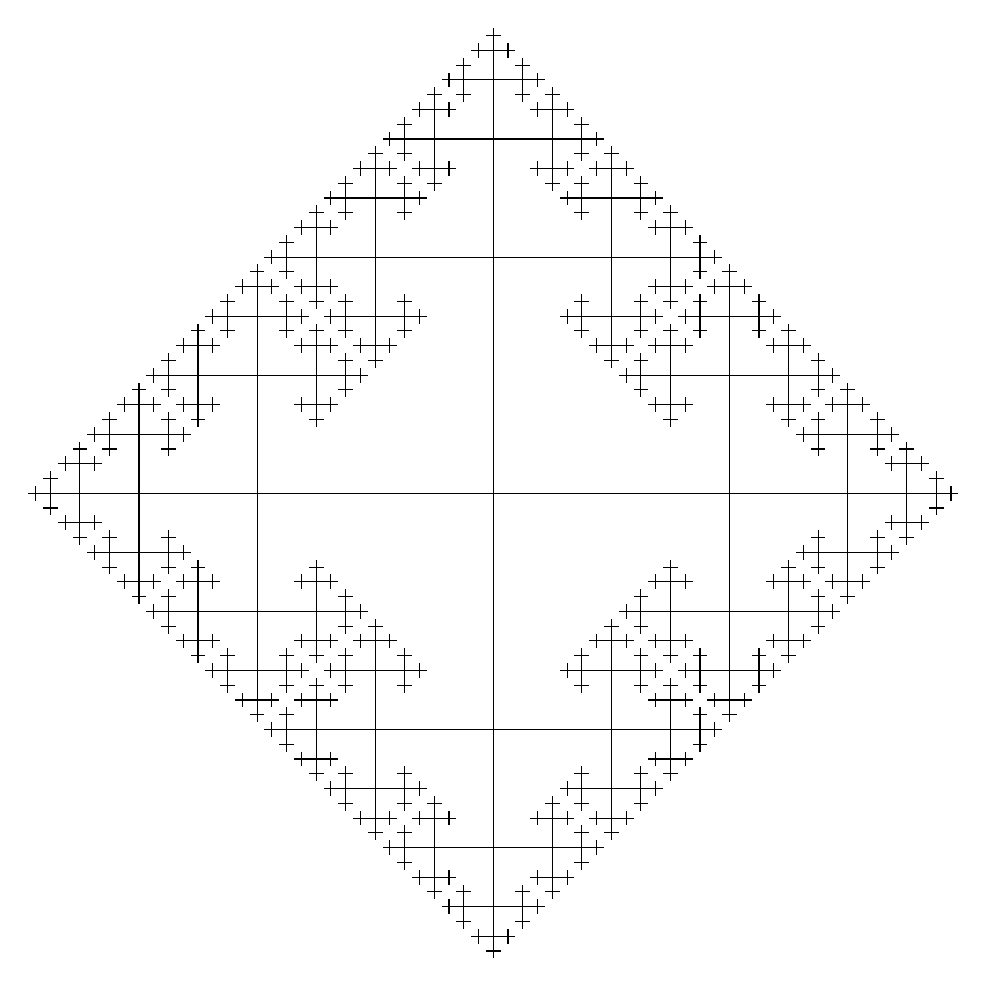
\begin{tikzpicture}
        \pgfdeclarelindenmayersystem{cayley}{
            \rule{F -> F [ R [F] [+F] [-F] ]}
            \symbol{R}{
                \pgflsystemstep=0.5\pgflsystemstep
            }
        }
        \draw l-system [l-system={cayley, axiom=[F] [+F] [-F] [++F], step = 3cm, order = 5}];
    \end{tikzpicture}

    只可意会的二阶自由群 Cayley 图
\end{center}

\subsection{自由交换群 (Free abelian group)}

自由交换群和自由群类似,只不过群变成了交换群:
\[
    \begin{tikzcd}
        \symscr{F} ^{\text{ab}}(A)\arrow[r, "\psi "] & G  \\
        A\arrow[u, "j"]\arrow[ur,"f"']               & {} \\
    \end{tikzcd}
\]
考虑 \(\symbb{Z} \) 的 \(n\) 次直积(在交换的前提下记为直和) \(\symbb{Z} ^{\oplus n}\),则面对元数数量为 \(n\) 的群 \(A\) 时,\(\symbb{Z} ^{\oplus n}\cong \symscr F^{\text{ab}}(A)\)。

\begin{proof}{\(\symbb{Z} ^{\oplus |A|}\cong \symscr F^{\text{ab}}(A)\)}
    \[
        \begin{tikzcd}
            \symbb{Z} ^{\oplus |A|}\arrow[r, "\psi "] & G  \\
            A\arrow[u, "j"]\arrow[ur,"f"']            & {} \\
        \end{tikzcd}
    \]
    \(j\) 定义为:
    \[
        j:a_i\mapsto (\underbrace{0,\cdots ,1}_i,\cdots ,0)
        .\]
    则我们可以仿照自由群那样让 \(j(a)\) 生成整个群(其实上也的确如此):
    \[
        +_{ \symbb{Z} ^{\oplus |A|}}: ((m_1,\cdots ,m_n),(k_1,\cdots ,k_n))\mapsto (m_1+k_1,\cdots ,m_n+k_n)
        .\]
    因此:
    \[
        (m_1,\cdots ,m_n) = \sum_{1\leqslant i\leqslant n} m_ij(a_i)
        .\]
    由于图表的交换性,那么有:
    \[
        \psi \left(   (\underbrace{0,\cdots ,1}_i,\cdots ,0) \right)  = f(a_i)
        .\]
    和群同态的性质——
    \[
        \psi((m_1,\cdots ,m_n)) = \prod_{1\leqslant i\leqslant n} f(a_i)^{m_i}
        .\]
    最后验证这确实是个群同态:
    \[
        \begin{aligned}
            \psi((m_1,\cdots ,m_n) + (k_1,\cdots ,k_n)) & = \psi ((m_1+k_1,\cdots ,m_n+k_n))                                                                                   \\
                                                        & =\prod_{1\leqslant i\leqslant n} f(a_i)^{m_i+k_i}                                                                    \\
                                                        & \xlongequal{\text{Abelian}}{} \prod_{1\leqslant i\leqslant n}f(a_i)^{m_i}\prod_{1\leqslant i\leqslant n}f(a_i)^{k_i} \\
                                                        & = \psi((m_1,\cdots ,m_n))  \psi((k_1,\cdots ,k_n))
        \end{aligned}
    \]
\end{proof}

在此之上,我们定义针对集合的群直和:
\begin{defi}{直和}
    设 \(H\) 是一个交换群,\(A\) 是一个集合,则 \(\Hom_{\SET}(A,H) = H^A\) 是一个交换群。直和是 \(H^A\) 的子集,定义如下:
    \[
        H^{\oplus A} \coloneqq  \left\{ f\in H^A: \left\vert \left\{ a\in A:f(a)\neq 0_H \right\} \right\vert  <\infty \right\}
        .\]
\end{defi}

这解决了不可数集合的自由群问题,如下:

\begin{itemize}
    \item 定义 \(J_a:A\to H^{\oplus A}, x\mapsto \begin{cases}
              1, & \text{if } x=a,     \\
              0, & \text{if } x\neq a.
          \end{cases}\)则我们可以将 \( H^{\oplus A}\) 中的元素以下表示:
          \[
              \sum_{a\in A} m_aJ_a
              .\]
          则显然有 \(\psi :\sum_{a\in A} m_aJ_a\mapsto \sum_{a\in A} m_af(a)\)。

          当然 \(m_a\) 只有有限个不为零。
\end{itemize}
\end{document}